\documentclass[14pt]{beamer}
\usepackage[T2A]{fontenc}
\usepackage[utf8]{inputenc}
\usepackage[english,russian]{babel}
\usepackage{amssymb,amsfonts,amsmath,mathtext}
\usepackage{cite,enumerate,float,indentfirst}
\usepackage{movie15}
\usepackage{listings}

\usepackage{wrapfig}


\graphicspath{{images/}}

\usetheme{Berlin}
\usecolortheme{dolphin}

\setbeamercolor{footline}{fg=blue}
\setbeamertemplate{footline}{
  \leavevmode%
  \hbox{%
  \begin{beamercolorbox}[wd=.333333\paperwidth,ht=2.25ex,dp=1ex,center]{}%
	  Шевкунов Кирилл, МФТИ
  \end{beamercolorbox}%
  \begin{beamercolorbox}[wd=.333333\paperwidth,ht=2.25ex,dp=1ex,center]{}%
	  Москва, 2018
  \end{beamercolorbox}%
  \begin{beamercolorbox}[wd=.333333\paperwidth,ht=2.25ex,dp=1ex,right]{}%
  стр. \insertframenumber{} из \inserttotalframenumber \hspace*{2ex}
  \end{beamercolorbox}}%
  \vskip0pt%
}

\newcommand{\itemi}{\item[\checkmark]}



\title{\small{Решающие деревья и ансамбли}}
\author{\small{%
	Шевкунов Кирилл
}\\%
\vspace{30pt}%
ФИВТ МФТИ
\vspace{20pt}%
}
\date{\small{Москва, 2018}}

\begin{document}

\newtheorem{rudef}{Определение}

\maketitle
\begin{frame}
\frametitle{План}
\begin{itemize}
  \item \textbf{Решающие деревья} 
	  \begin {itemize}
		\item Терминология
		\item Дерево как классификатор
		\item Дерево как регрессор
		\item Построение деревьев
	  \end {itemize}
  \item \textbf{Случайный лес} 
	  \begin {itemize}
		\item Идея ансамблирования
		\item Алгоритм
	  \end {itemize}
  \item \textbf{Градиентный бустинг} 
	  \begin {itemize}
		\item Идея
		\item Градиентный спуск
		\item Алгоритм
	  \end {itemize}
\end{itemize}
\end{frame} 

\begin{frame}
	\frametitle{Терминология}
	
	\begin{rudef}
        Граф - множество вершин и рёбер между ними
    \end{rudef}
    \pause
    
	\begin{rudef}
        Дерево - связный граф без циклов
    \end{rudef}
    \pause
    
 	\begin{rudef}
        Лес - граф состоящий из несвязанных деревьев (любой граф без циклов)
    \end{rudef}
\end{frame}

\begin{frame}
\frametitle{Пример с разделимыми выборками}

    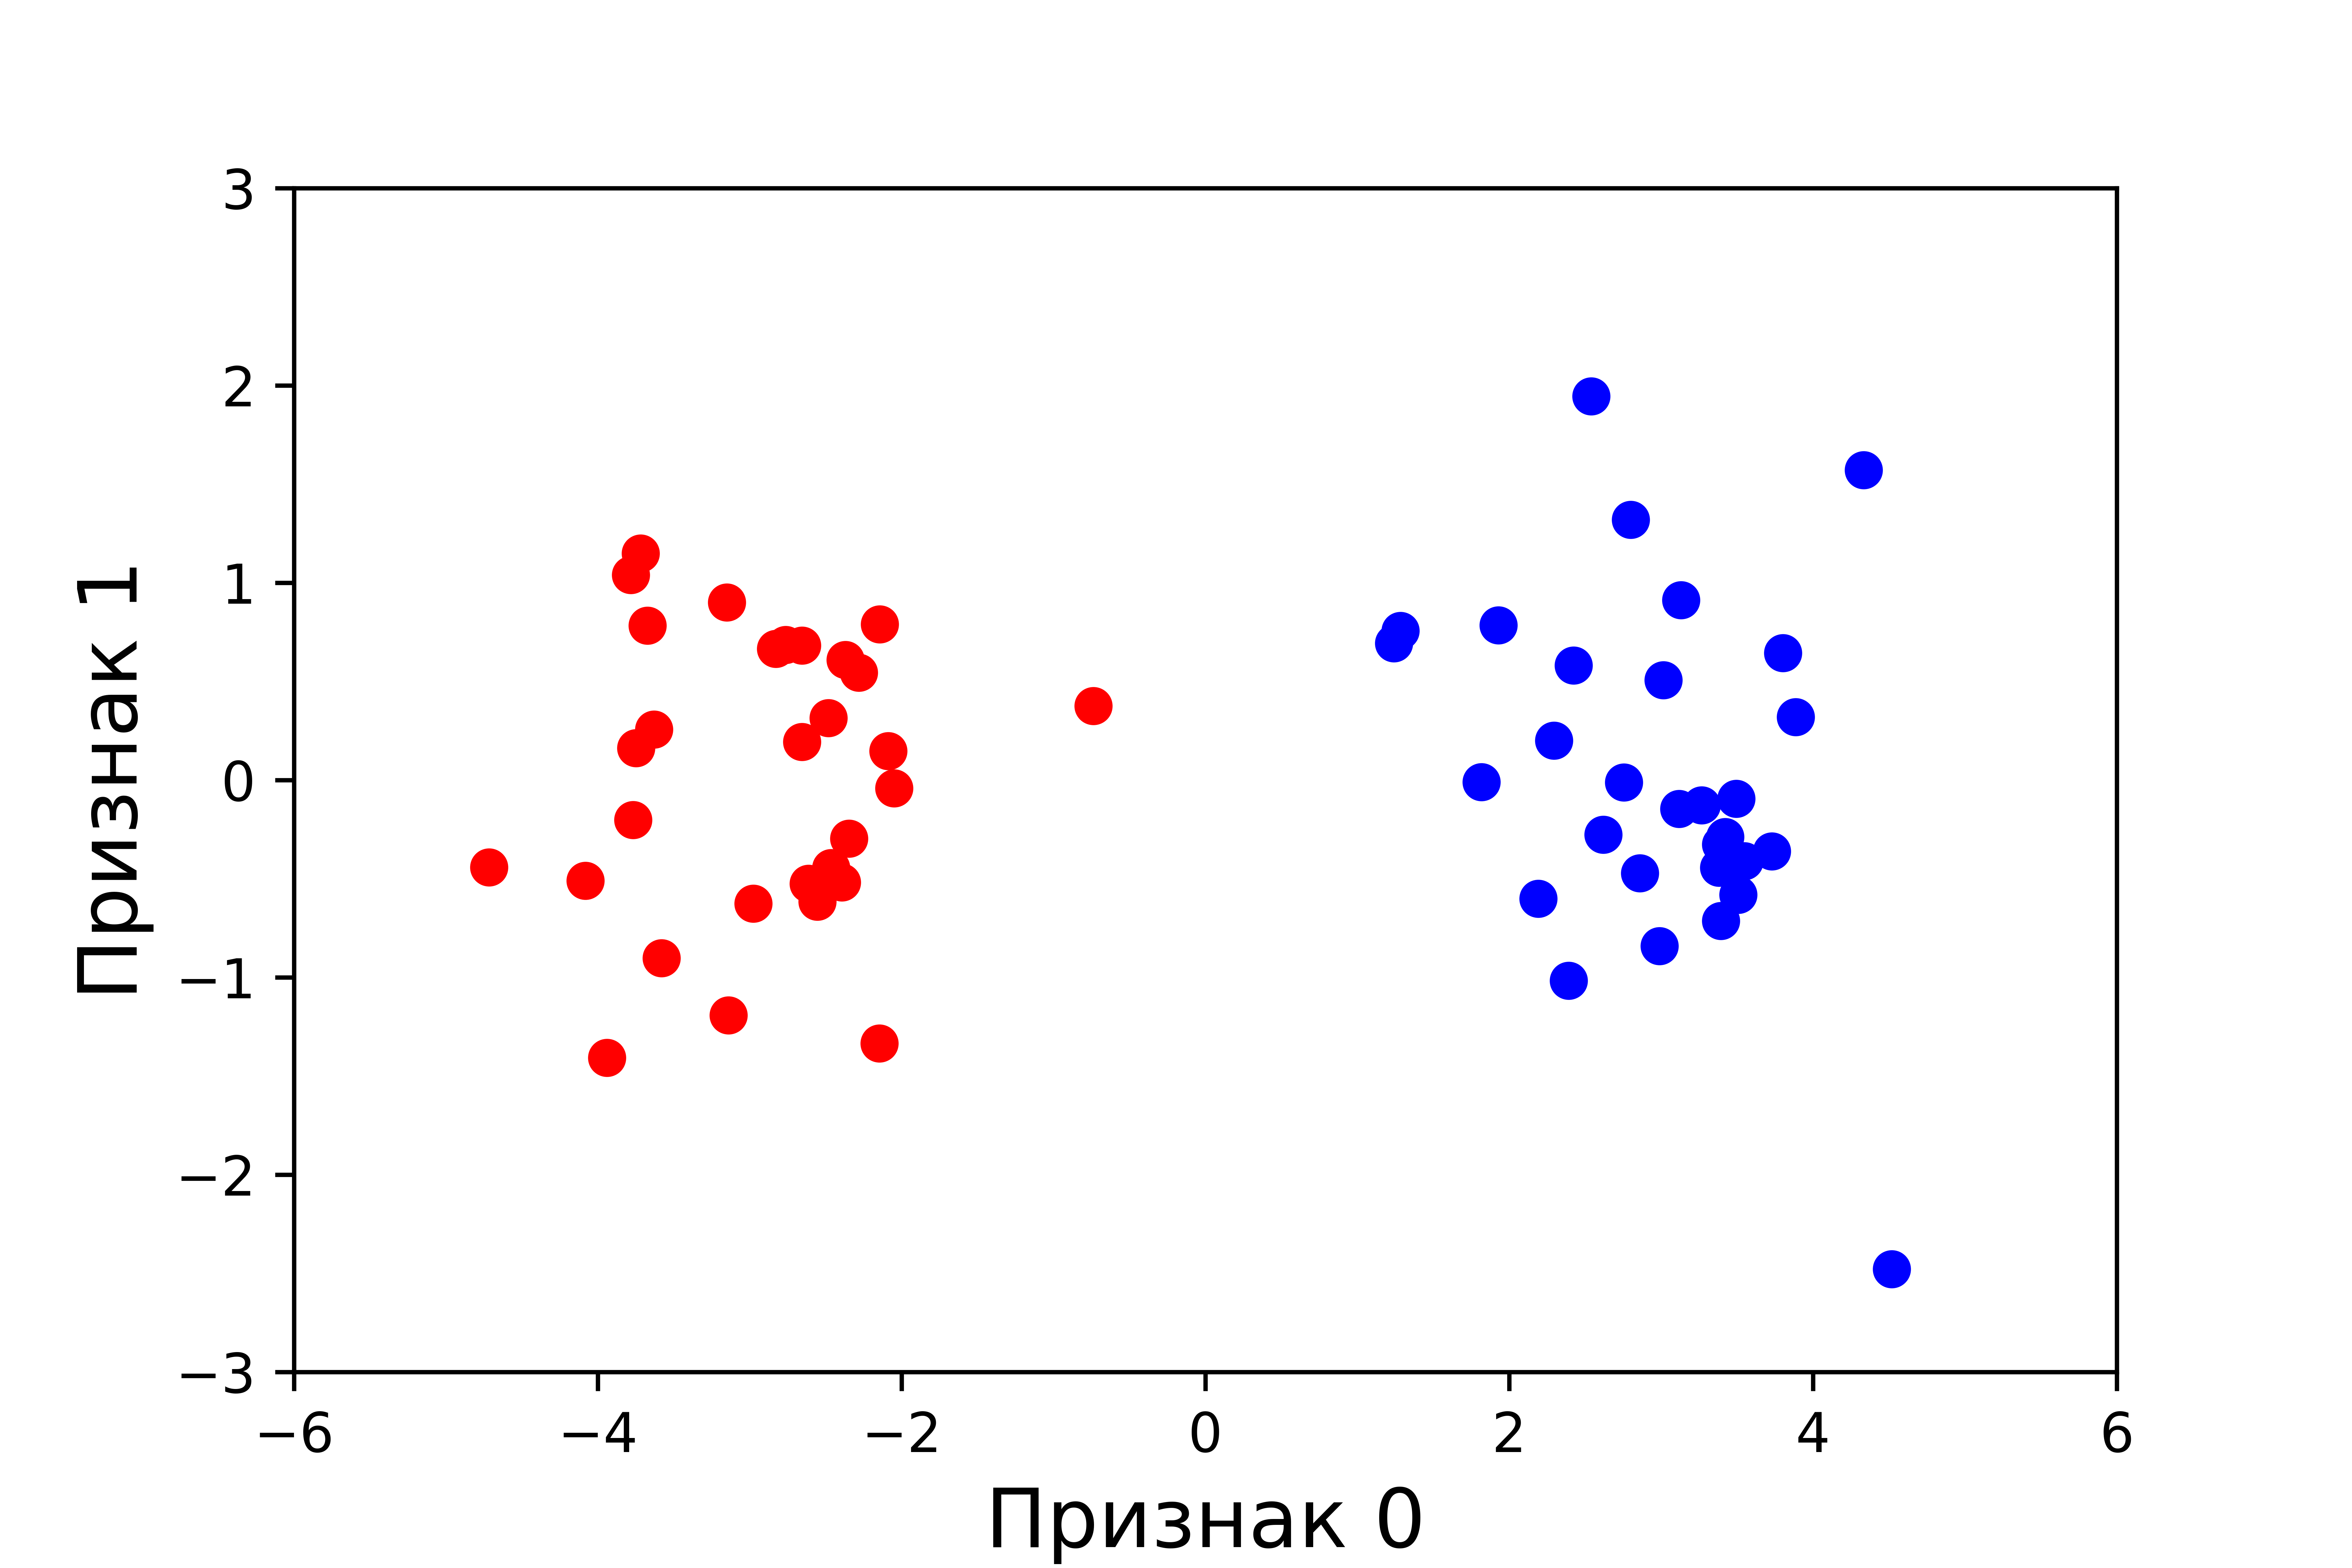
\includegraphics[width=0.5\textwidth]{tree_one_feature_separable.png}   
    \pause
    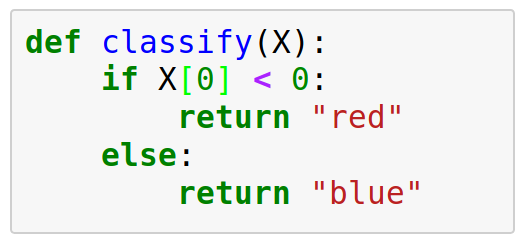
\includegraphics[width=0.5\textwidth]{tree_one_feature_separable_classifier.png}   

\end{frame}

\begin{frame}
\frametitle{Пример с разделимыми выборками}

    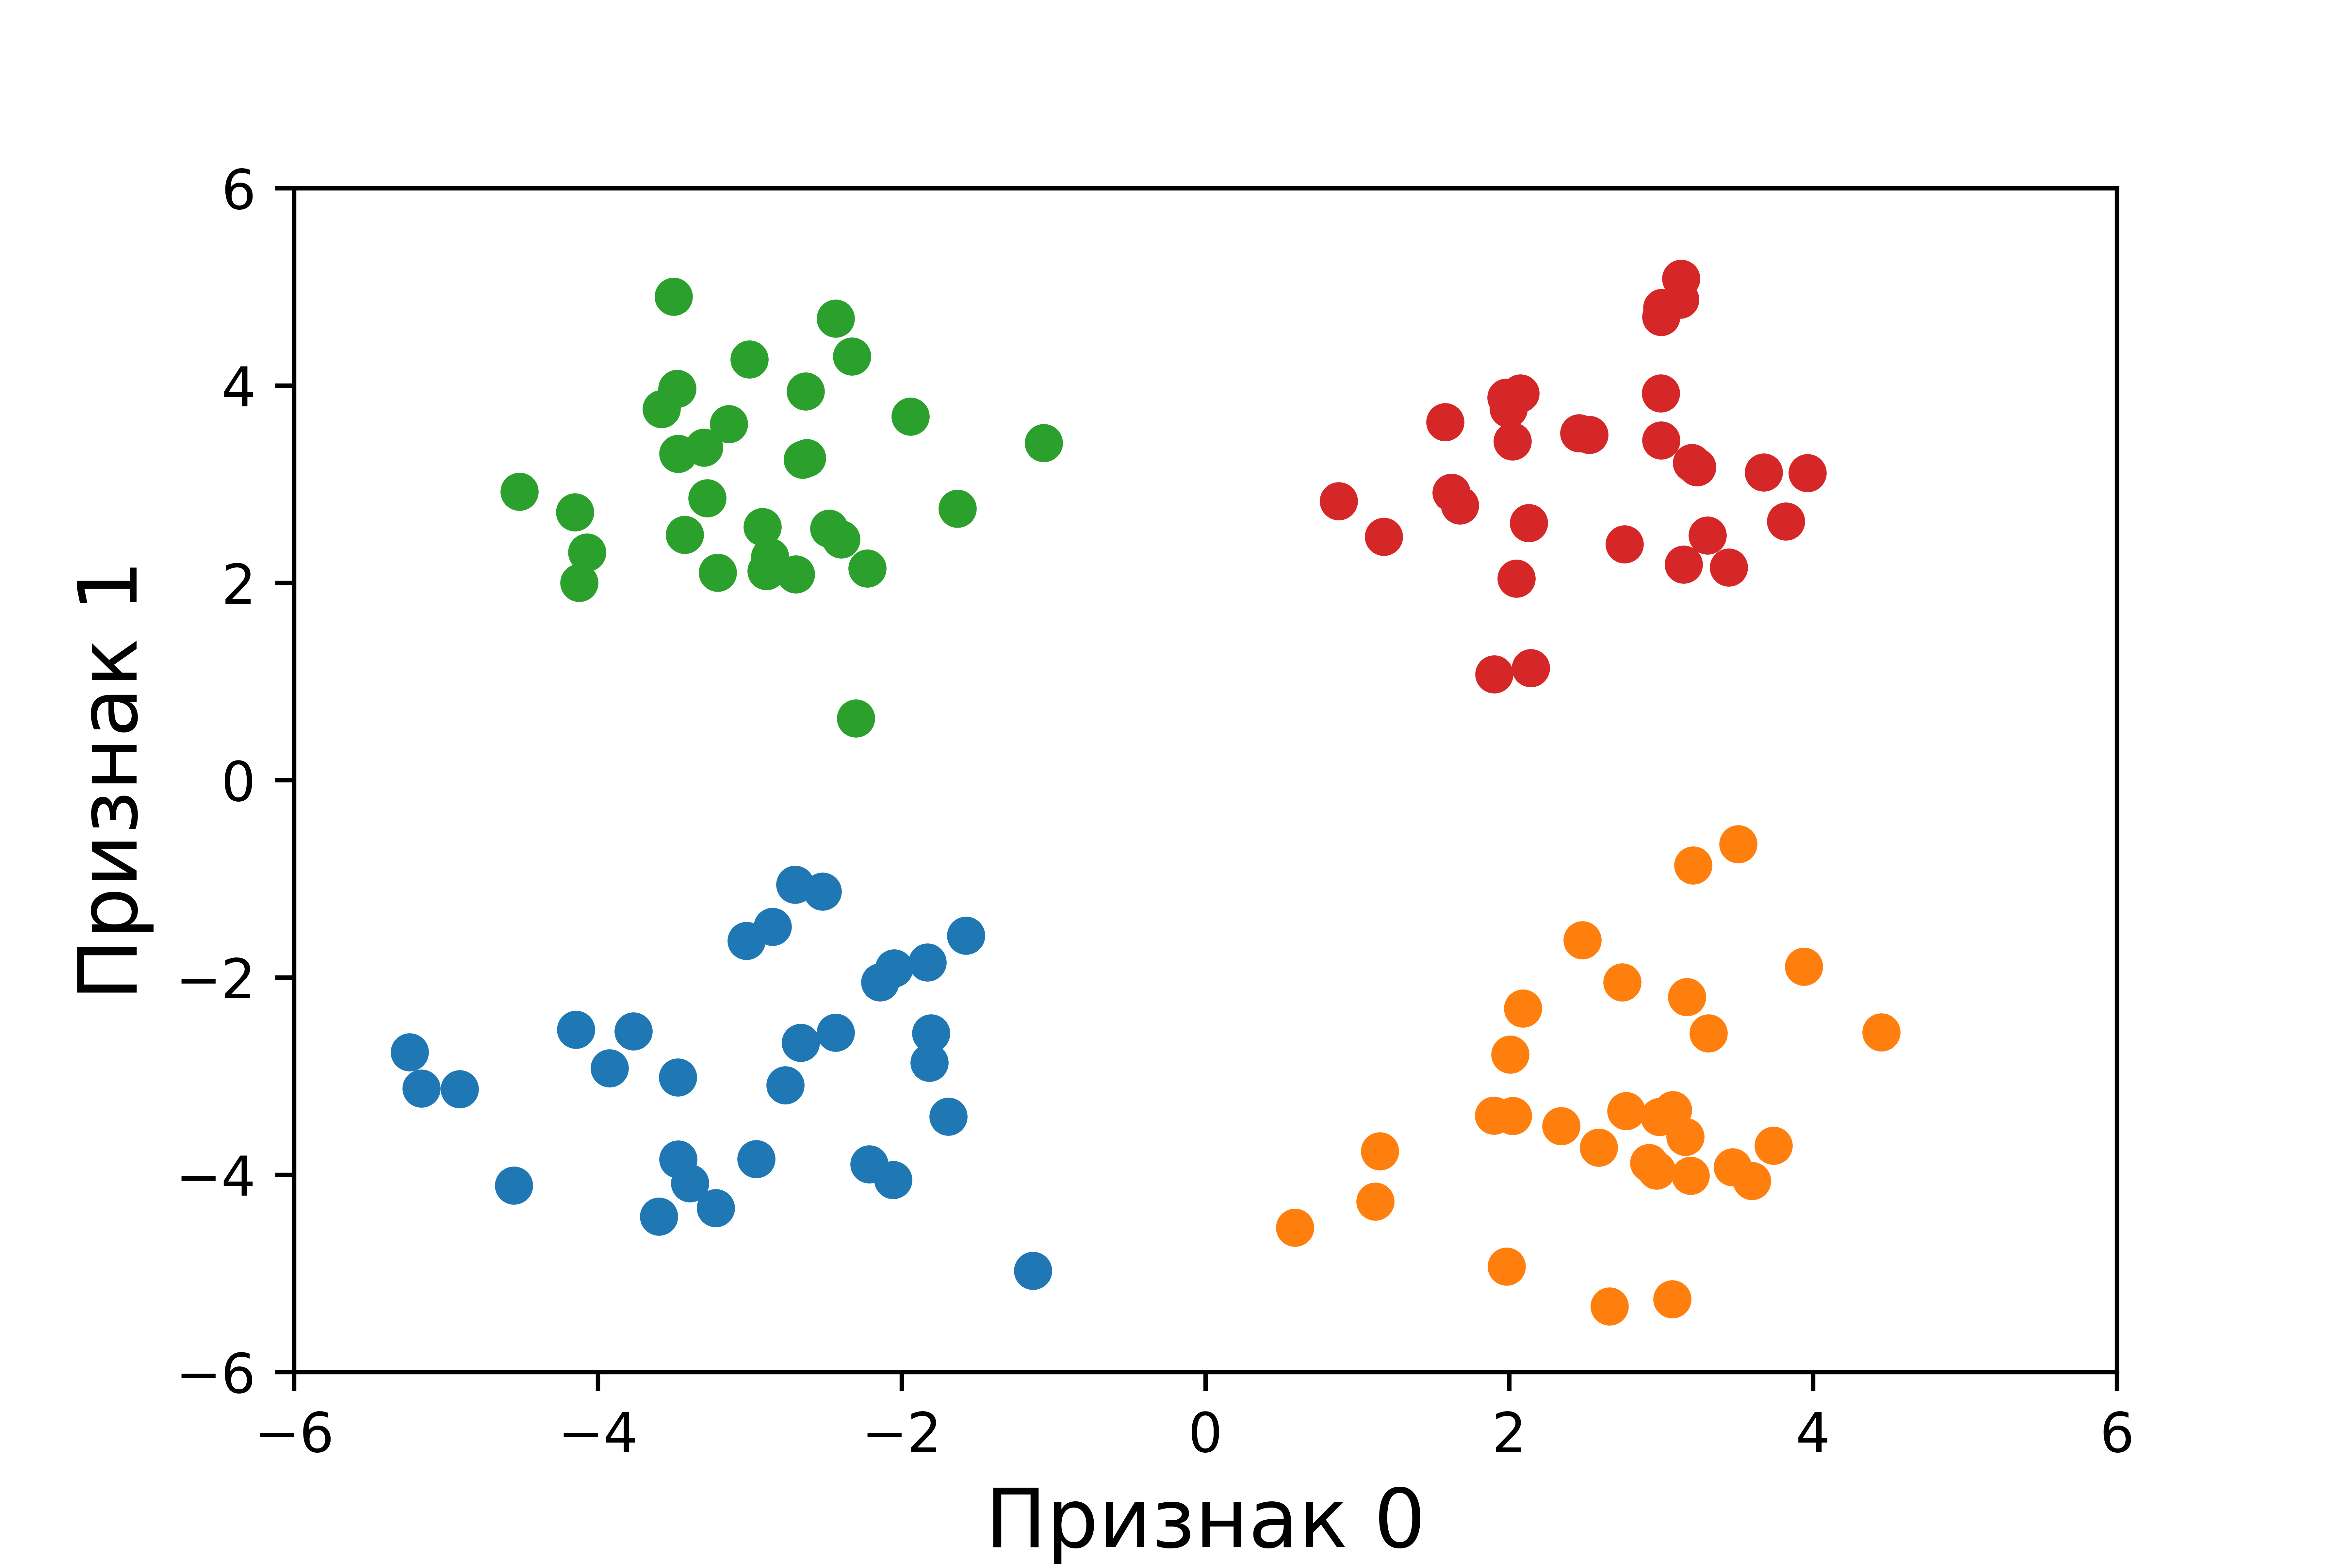
\includegraphics[width=0.5\textwidth]{tree_two_features_separable.png}
    \pause
    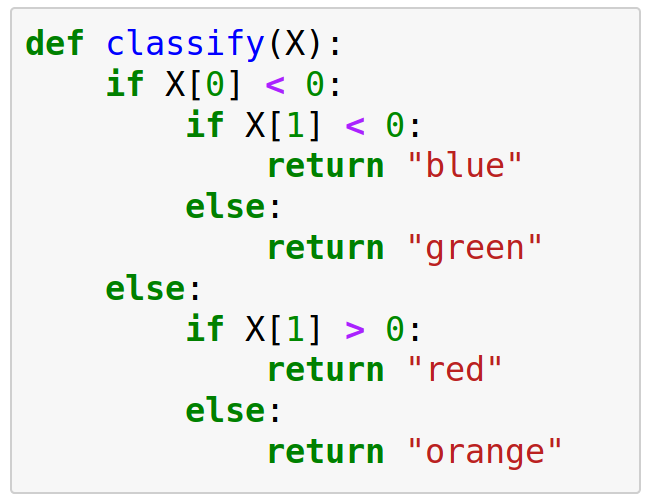
\includegraphics[width=0.5\textwidth]{tree_two_features_separable_classifier.png}   

\end{frame}


\begin{frame}
\frametitle{Решающее дерево}
    \begin{center}
        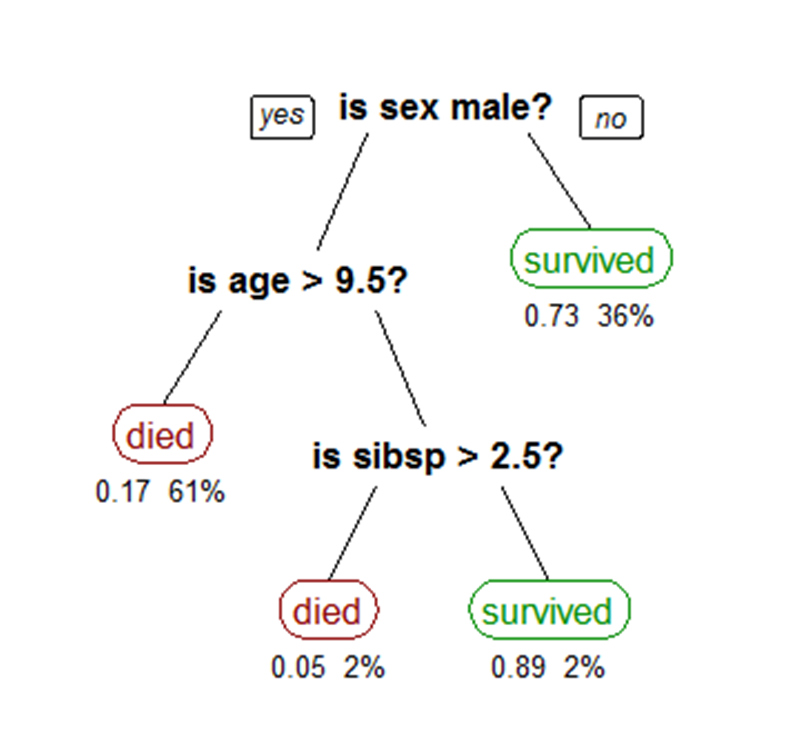
\includegraphics[width=0.6\textwidth]{tree_titanic.jpg} 
    \end{center}

\end{frame}

\begin{frame}
\frametitle{Решающее дерево для регрессии}
    \begin{center}
        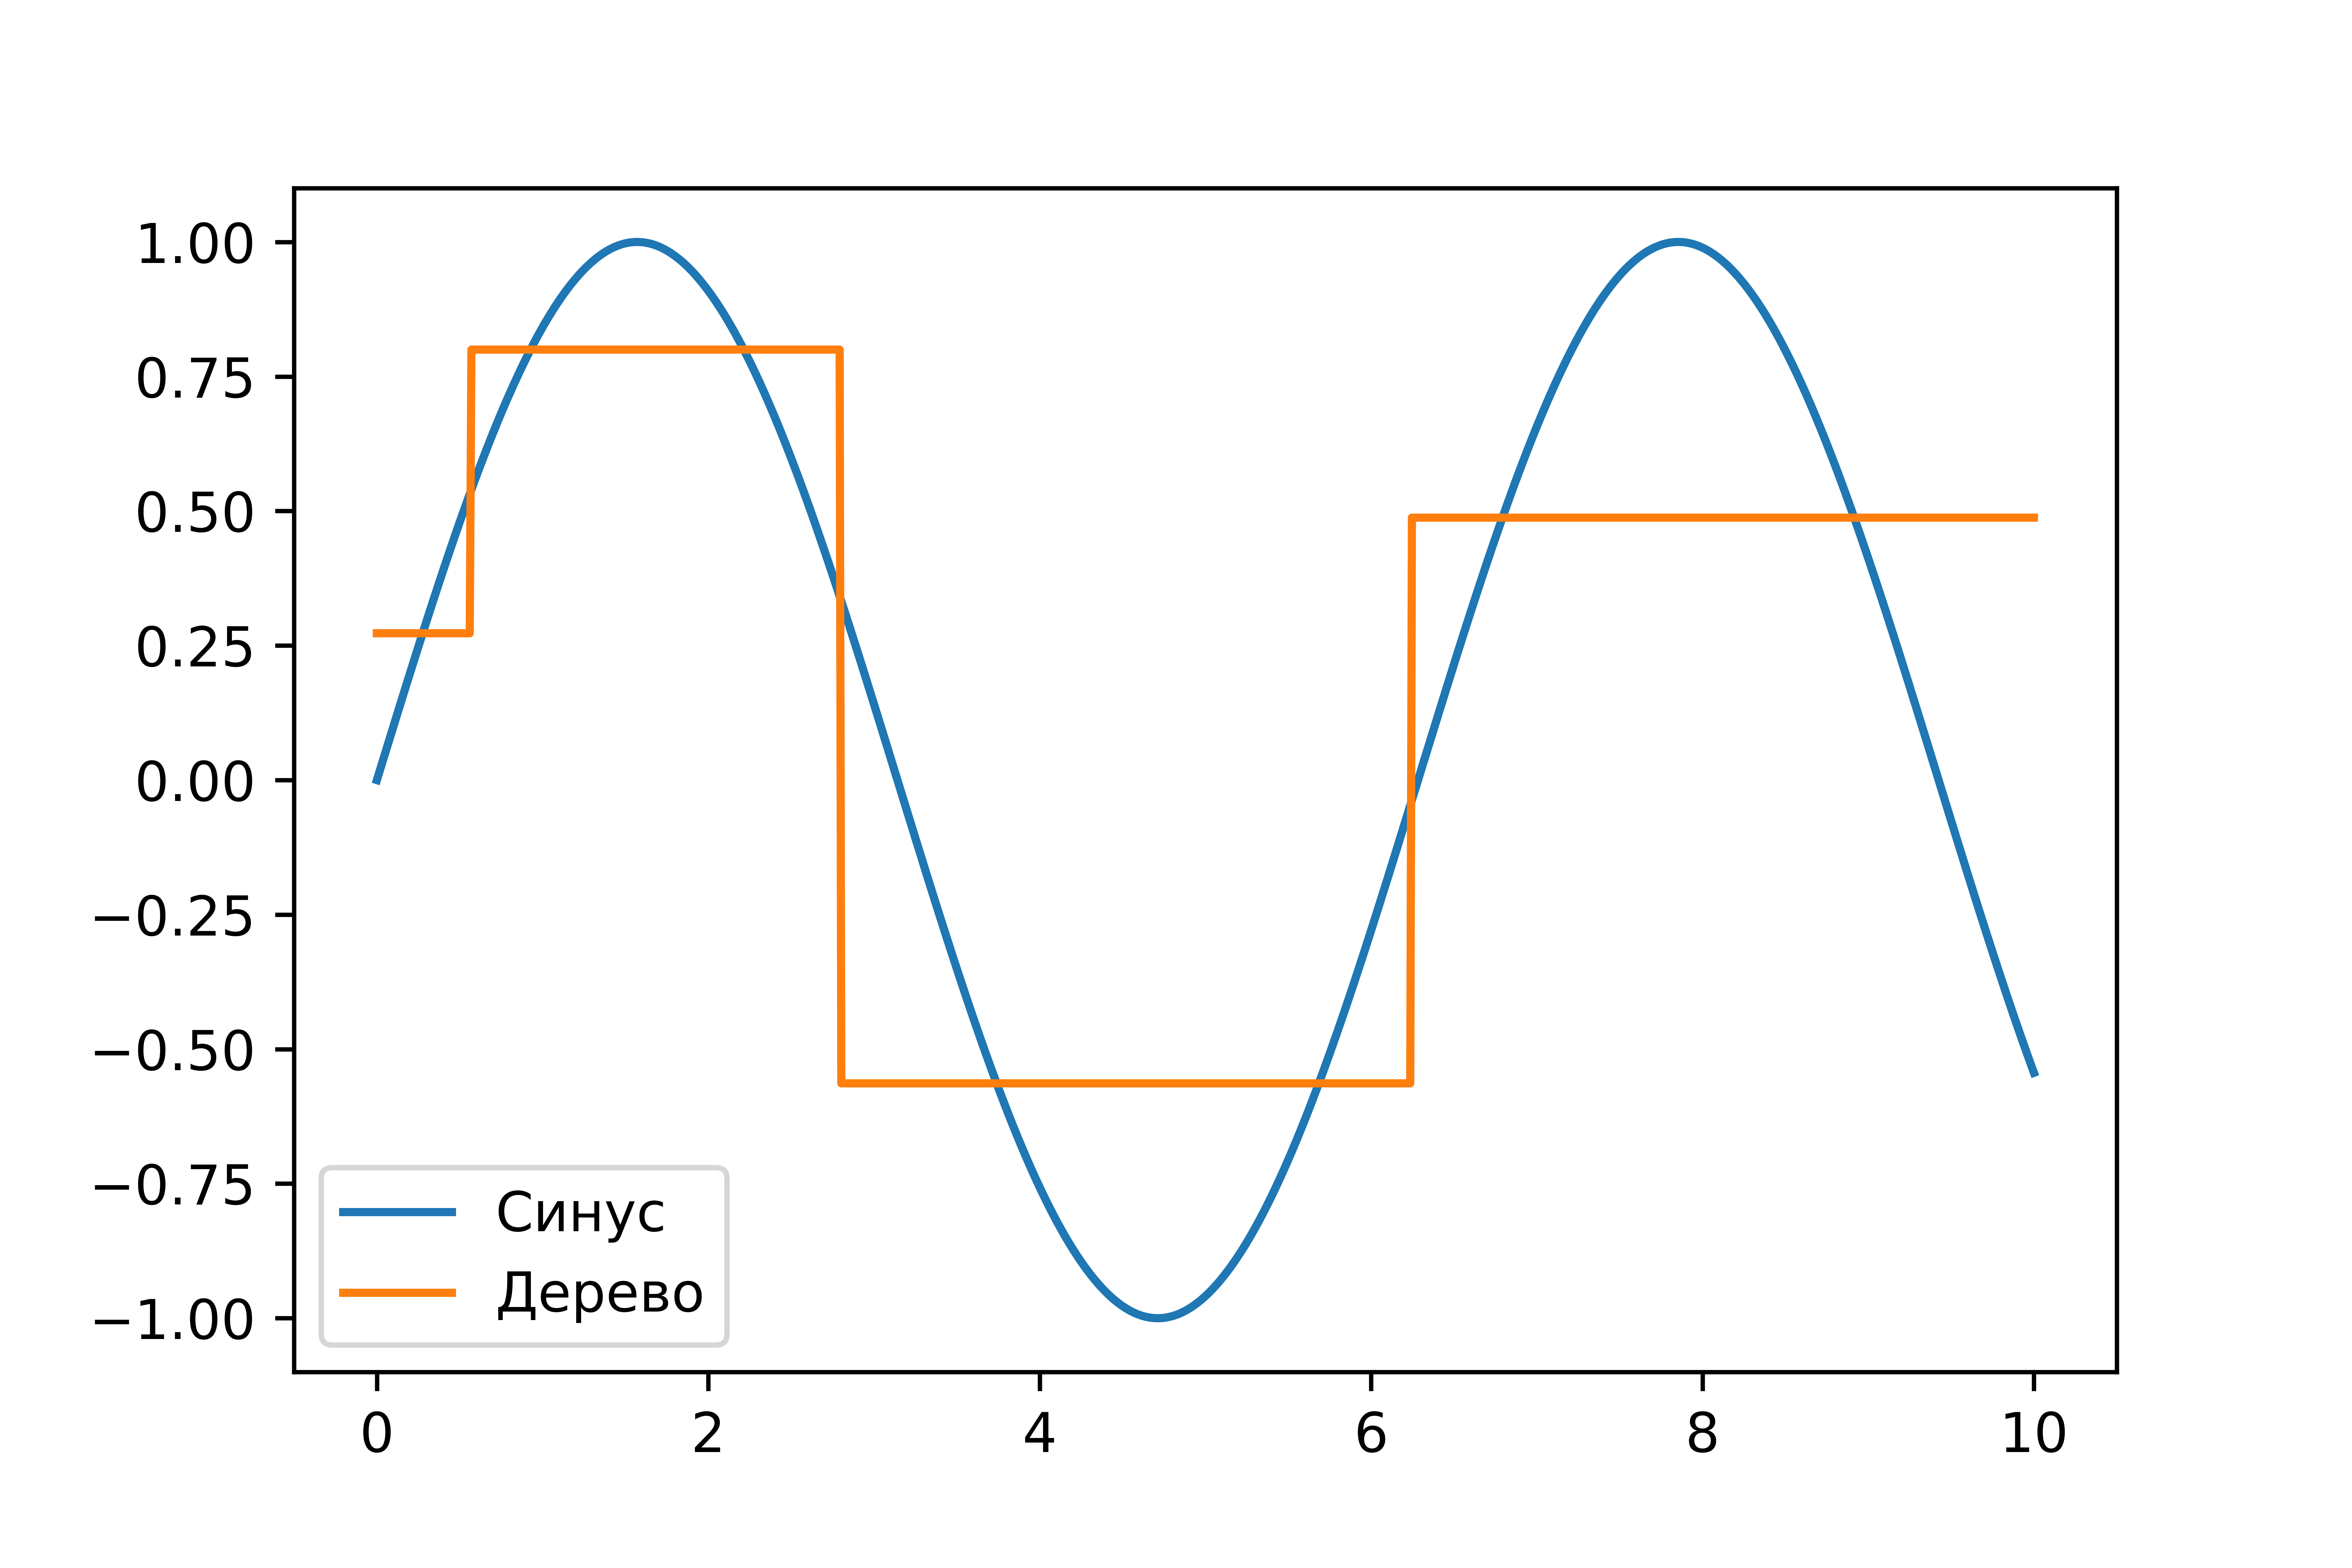
\includegraphics[width=0.5\textwidth]{tree_sinus.png}
        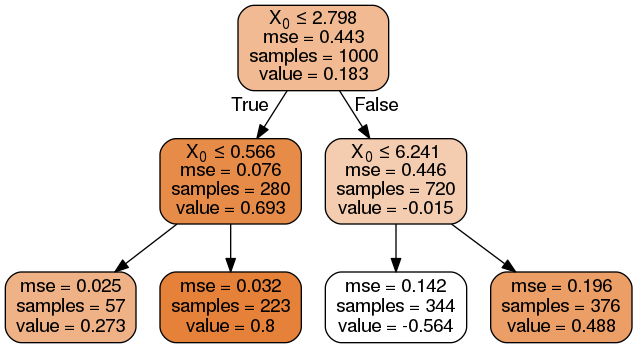
\includegraphics[width=0.5\textwidth]{tree_sinus_tree.png}
    \end{center}
    
\end{frame}

\begin{frame}
\frametitle{Разделяющая кривая и переобучение}
	\vspace{-1em}
    \begin{center}
        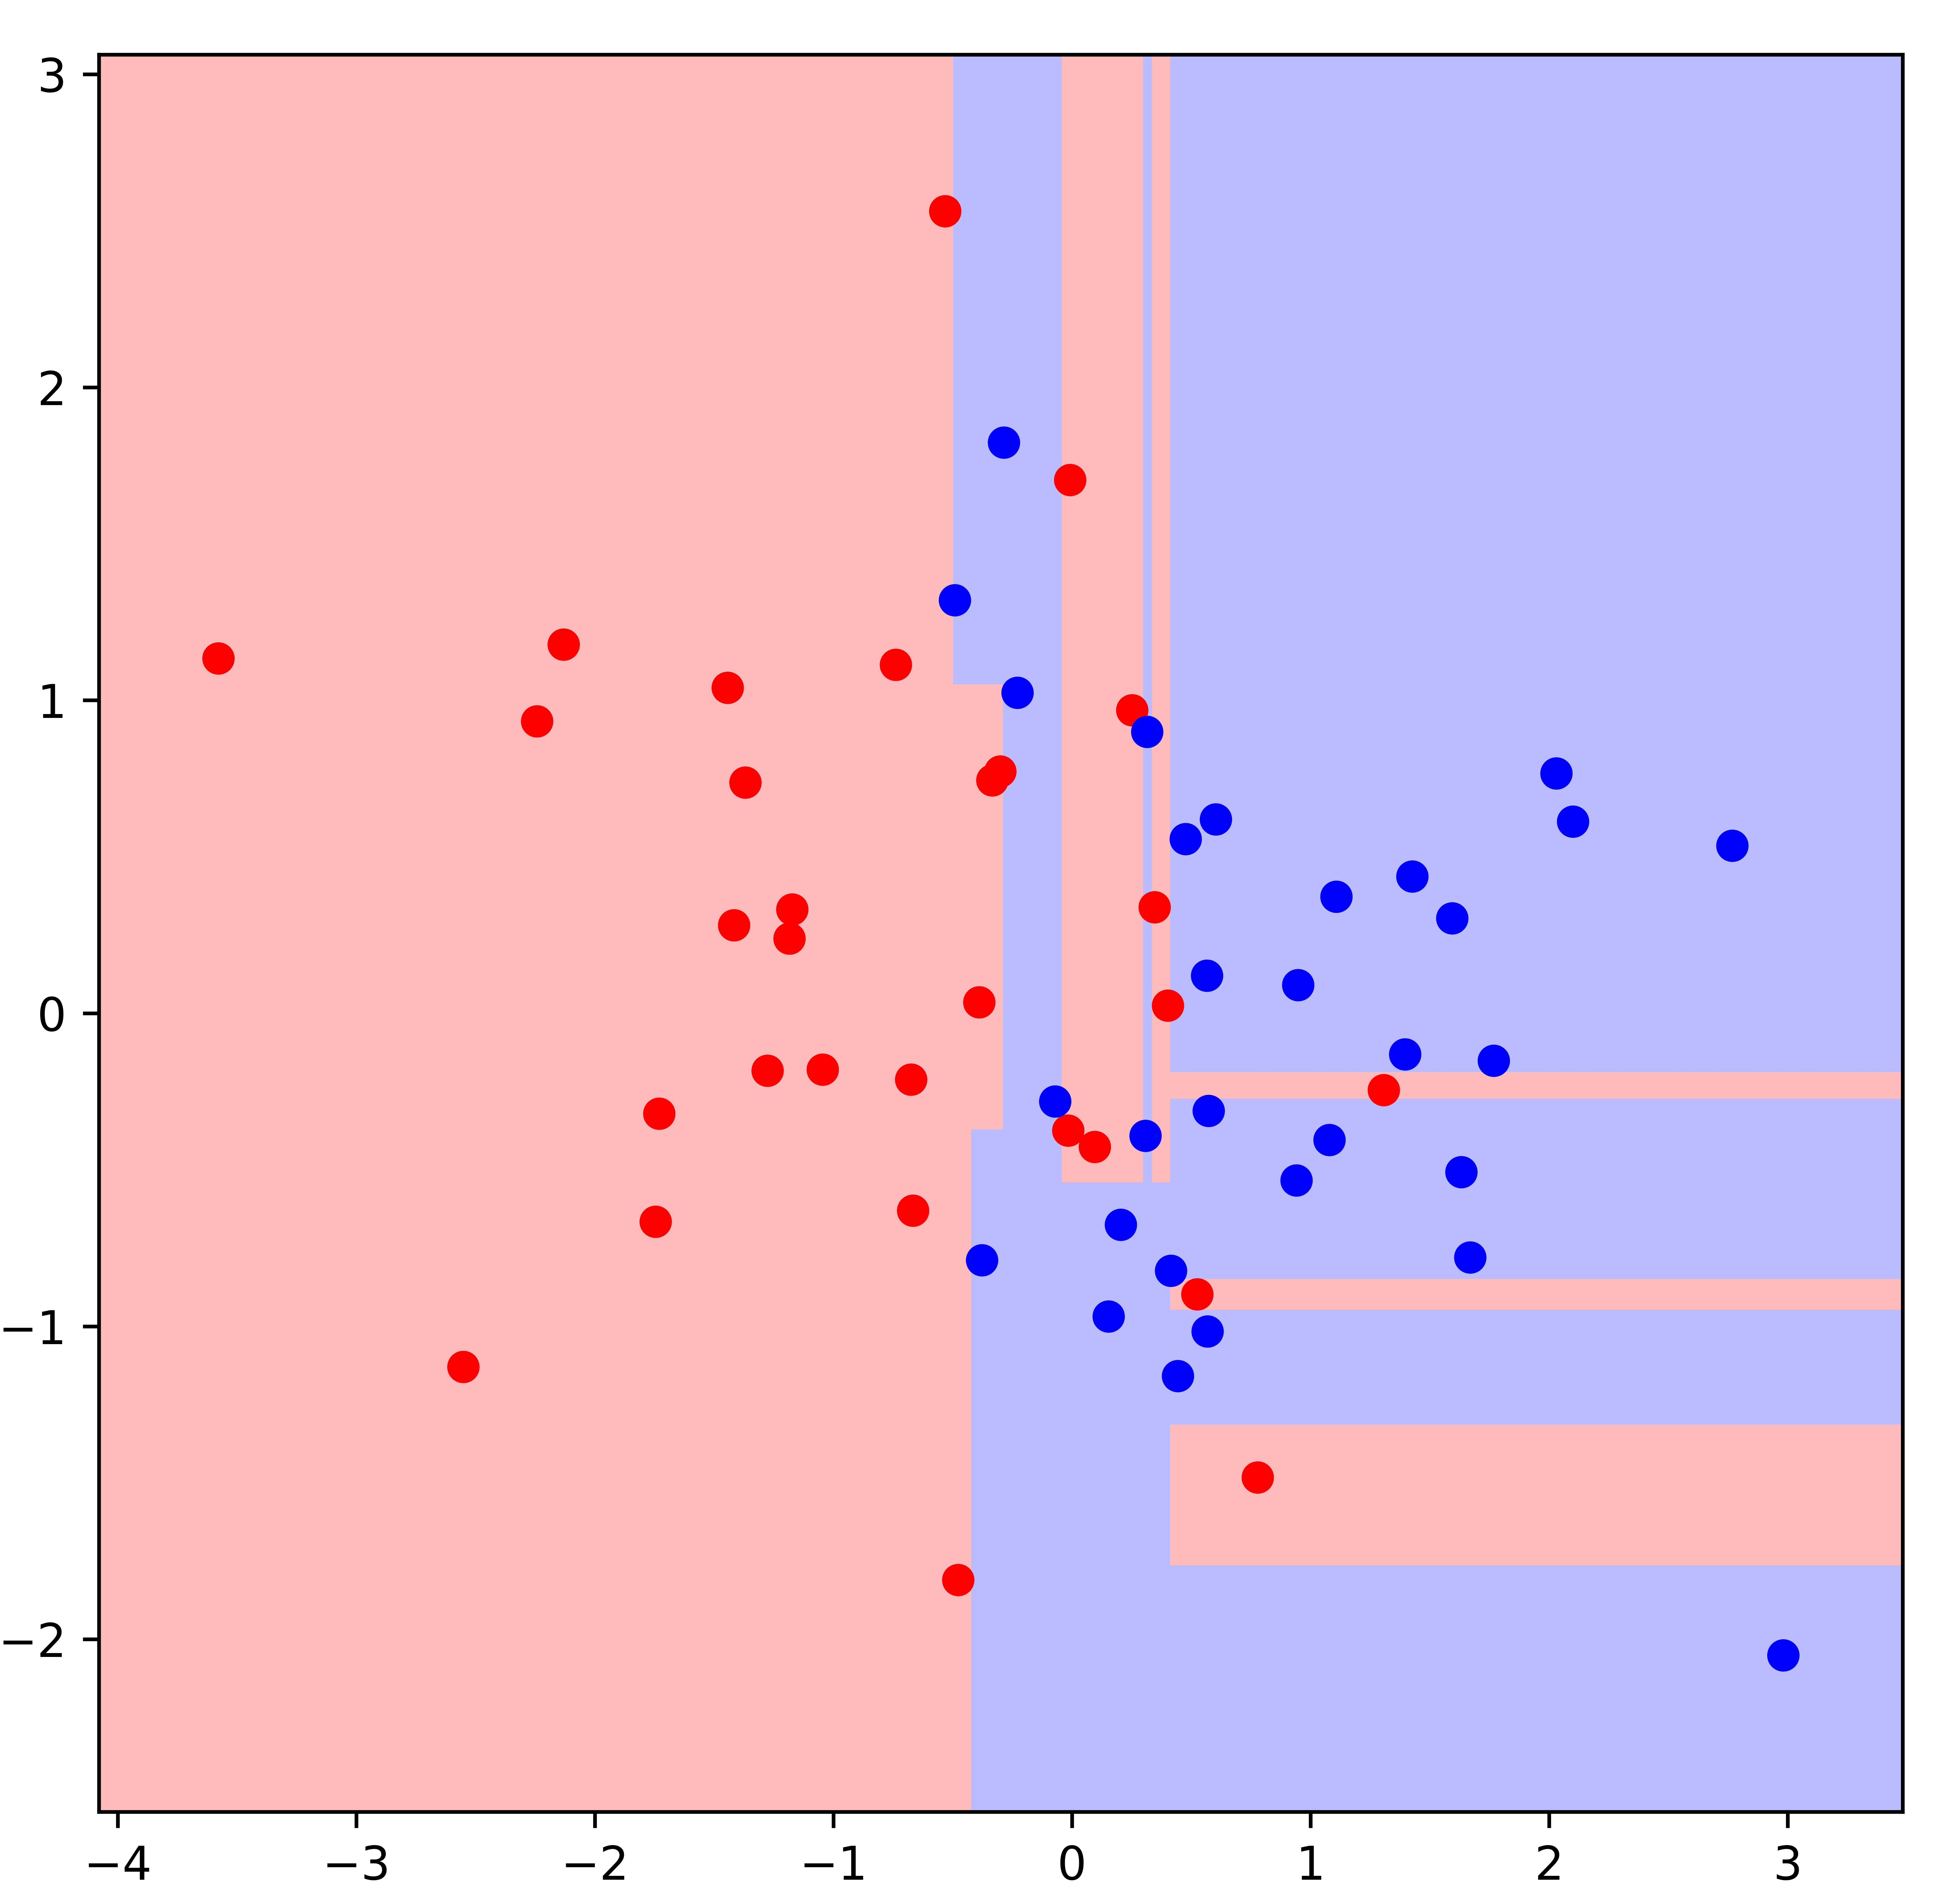
\includegraphics[width=0.6\textwidth]{tree_colormesh_1.png}
    \end{center}
\end{frame}

\begin{frame}
\frametitle{Разделяющая кривая и переобучение}
	\vspace{-1em}
    \begin{center}
        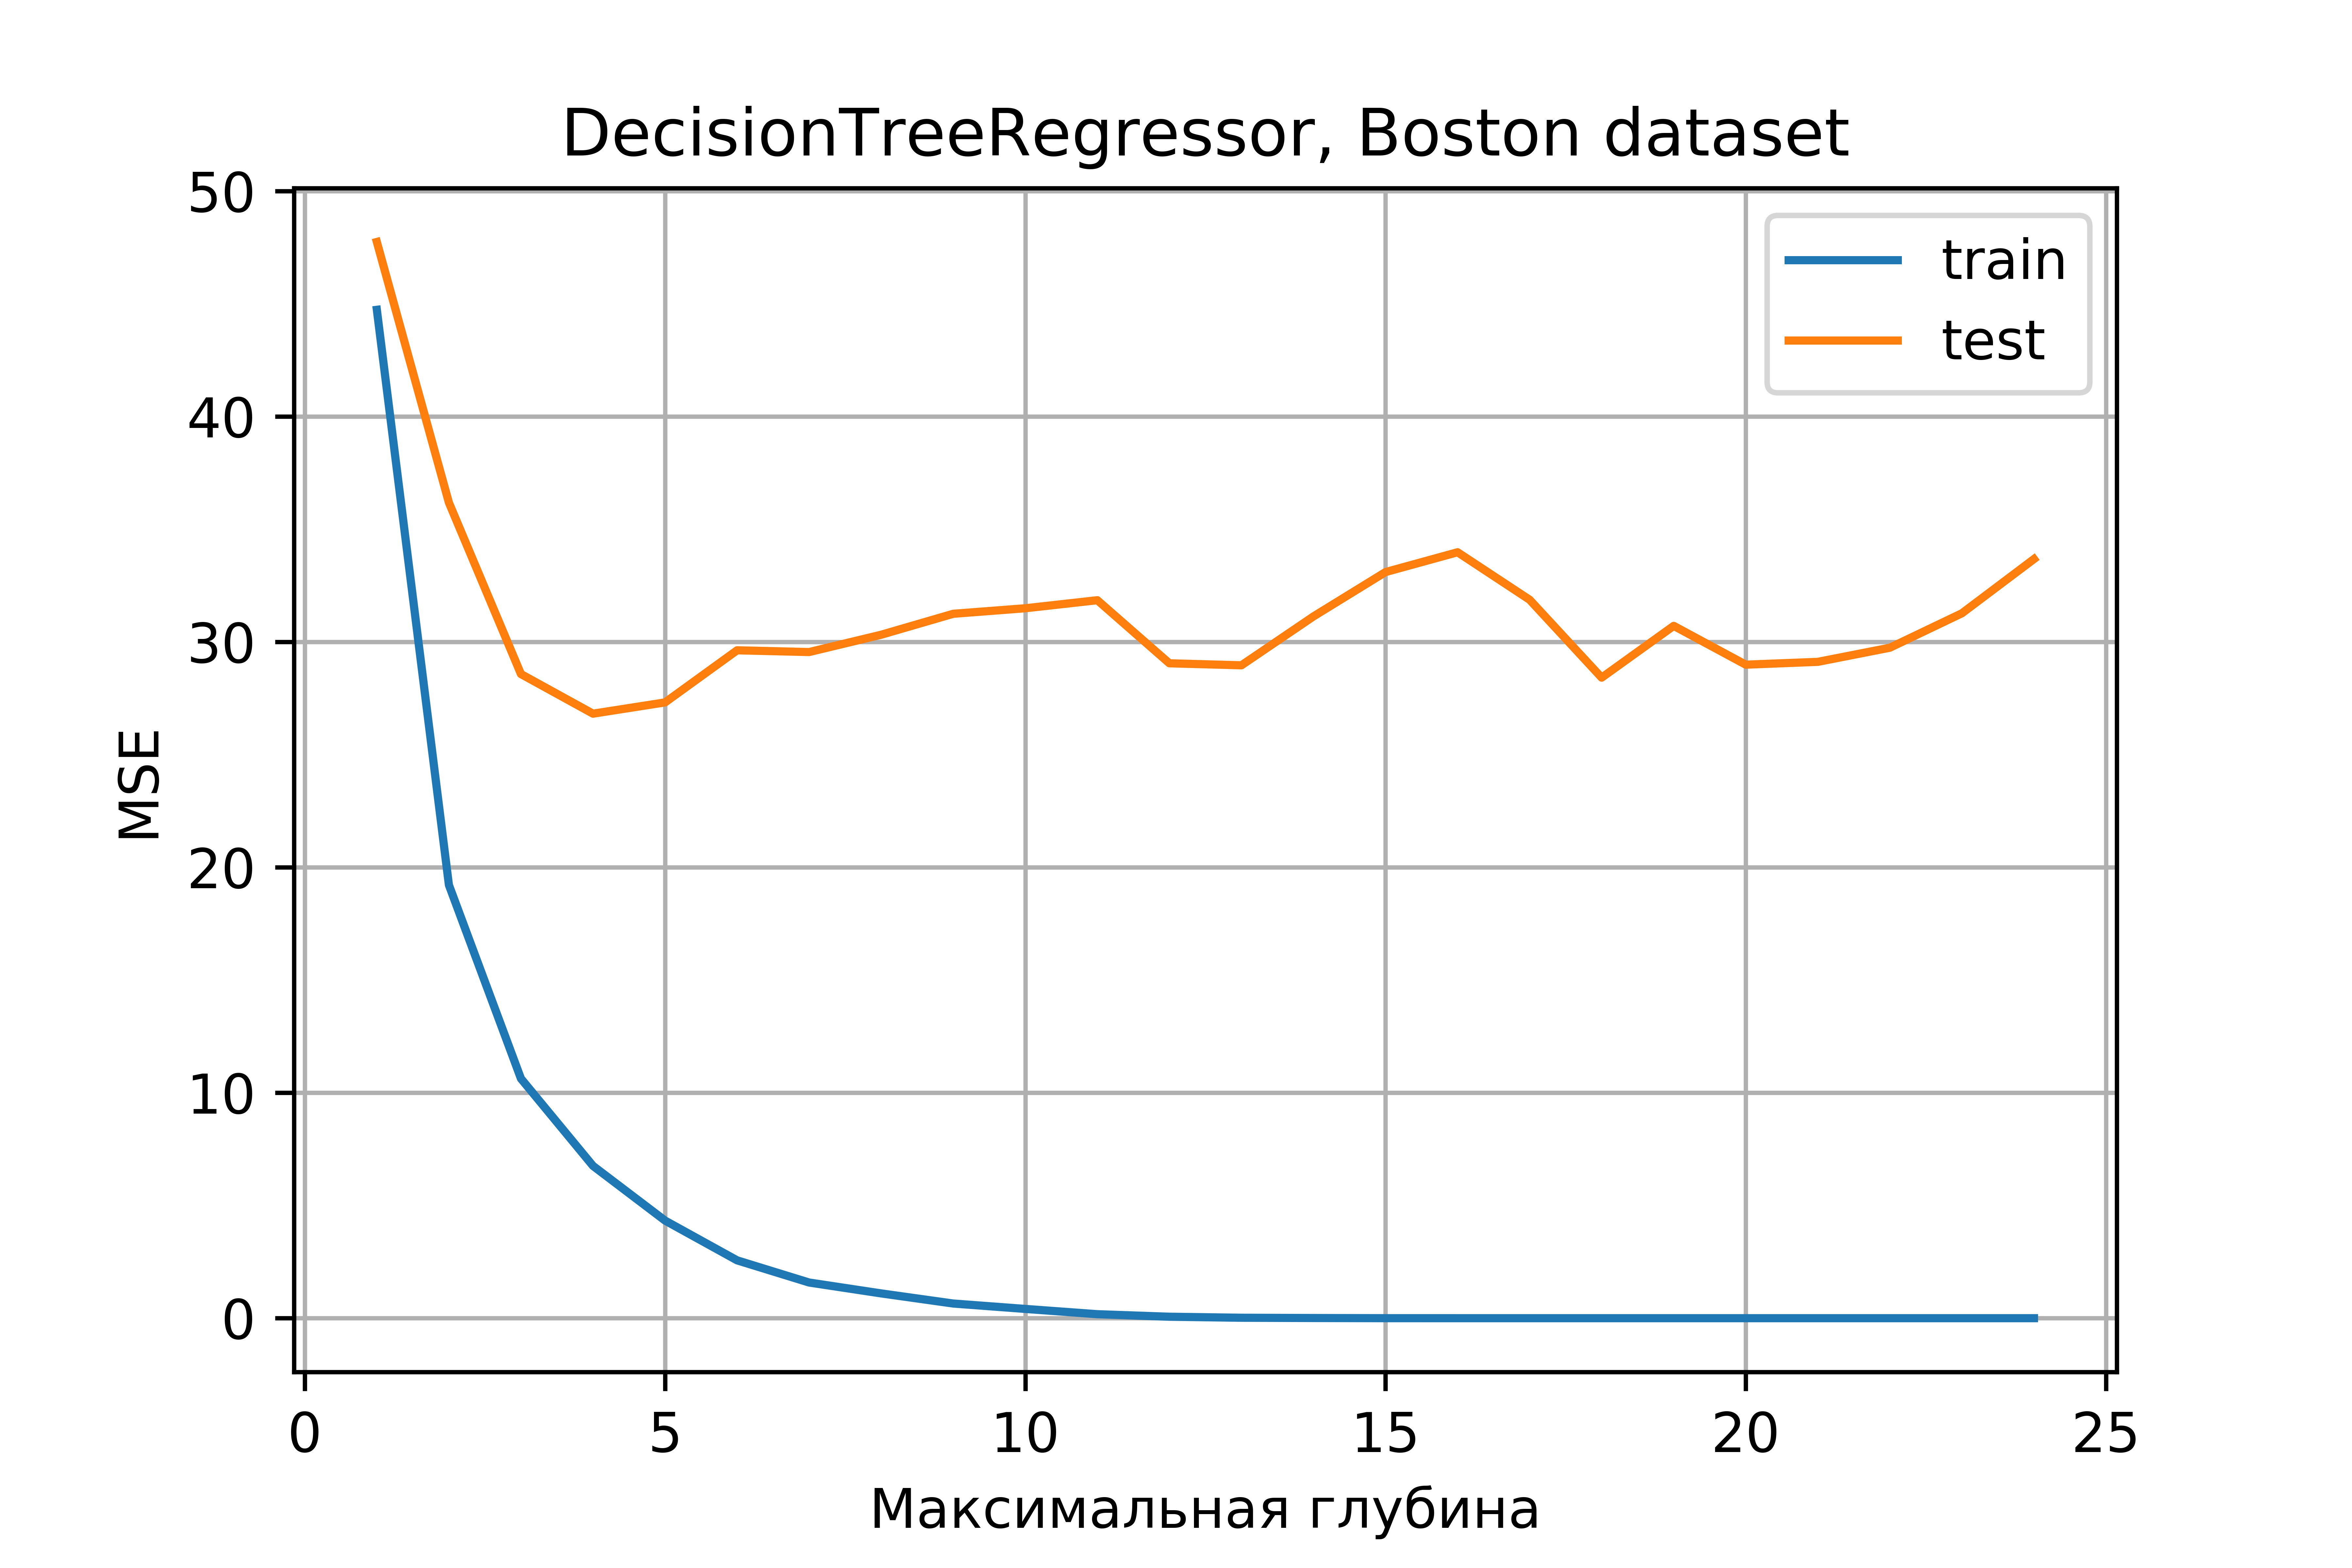
\includegraphics[width=0.8\textwidth]{tree_overfitting.png}
    \end{center}
\end{frame}

\begin{frame}
\frametitle{Построение дерева}
	\begin{rudef}
        Индекс неоднородности - величина, оценивающая неоднородность выборки.
    \end{rudef}
    
    Для регрессии:
    \begin {itemize}
		\item MSE: $H(Y) = \frac{1}{|Y|} \sum\limits_{i=1}^{|Y|} (y_i - \overline{y})^2$ \\
		 $\overline{y} = \frac{1}{|Y|} \sum\limits_{i=1}^{|Y|} y_i$
	  \end {itemize}
\end{frame}

\begin{frame}
\frametitle{Построение дерева}

    Для классификации ($P_i$ - доля класса i в X, L - число классов):
    \begin {itemize}
    	\item Энтропия: $H(X) = -\sum\limits_{i=1}^{L} P_i \log{ P_i }$
    	\item Джини:  $H(X) = \sum\limits_{i=1}^{L} P_i (1 - P_i)$
    	\item Misclassification:   $H(X) = 1 - \max\limits_{1..L} P_i$
      \end {itemize}
      
    Замечание: нужно считать, что $P_i log(P_i) = 0$ при $P_i = 0$ 
\end{frame}

\begin{frame}
\frametitle{Построение дерева}

    Для классификации ($P_i$ - доля класса i в X, L - число классов):
    \begin {itemize}
    	\item Энтропия: $H(X) = -\sum\limits_{i=1}^{L} P_i \log{ P_i }$
    	\item Джини:  $H(X) = \sum\limits_{i=1}^{L} P_i (1 - P_i)$
    	\item Misclassification:   $H(X) = 1 - \max\limits_{1..L} P_i$
      \end {itemize}
      
    Замечание: нужно считать, что $P_i log(P_i) = 0$ при $P_i = 0$ 
\end{frame}

\begin{frame}
\frametitle{Построение дерева}

	\begin{rudef}
        Уменьшение среднего индекса неоднородности при разбиении:
        $I(Q, f, v) = H(Q) - \frac{|L|}{|Q|} H(L) - \frac{|R|}{|Q|} H(R)$
        
        
        Q - выборка, f - признак, v - порог, L и R - соответсвующие им разбиения выборки Q на две части.
    \end{rudef}
\end{frame}

\begin{frame}
\frametitle{Построение дерева}
	  \begin {itemize}
		\item Будем строить дерево от корня (стартовая вершина) к листьям (вершины, из которых некуда идти)
		\item В начале в стартовой вершине лежит вся выборка
	  \end {itemize}
\end{frame}

\begin{frame}
\frametitle{Построение дерева}
	  \begin {itemize}
	    \item Если в текущей вершине выполнен критерий останова - ничего не делаем в этой вершине.
		\item Выбрать f и v так, чтобы $I(Q, f, v)$ было максимально, например, перебрав все признаки и пороги.
		\item Разделим данную выборку на L и R согласно выбранным f и v, создадим двух потомков текущей вершиы и положим в них L и R соответственно.
		\item Повторим для каждой дочерней вершины.
	  \end {itemize}
\end{frame}

\begin{frame}
\frametitle{Варианты критериев останова}
	  \begin {itemize}
		\item Максимальная глубина дерева.
		\item Минимальный размер выборки в вершине.
		\item Все обьекты в ввершине одного класса
		\item Требование на функционал качества вида "улучшился на k процентов"
	  \end {itemize}
\end{frame}


\begin{frame}
\frametitle{Дополнительно}
	  \begin {itemize}
		\item Построенные деревья можно уменьшать, пытаясь улучшить качество - "стрижка деревьев". Используется в алгоритмах C4.5 и CART построения деревьев.
		\begin{center}
		    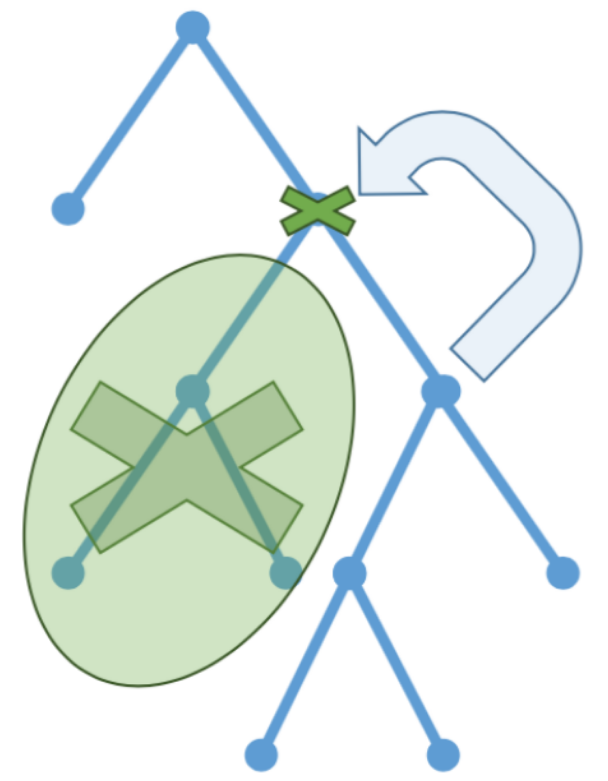
\includegraphics[height=0.5\textheight]{tree_pruning.png}
		\end{center}
	  \end {itemize}
\end{frame}

\begin{frame}
\frametitle{Дополнительно}
	  \begin {itemize}
		\item Деревья малой глубины легко интерпретируемы человеком, из-за чего часто применяются, например, в банковской сфере, т.к. доверять "чёрному ящику" деньги сложнее.
		\begin{center}
		    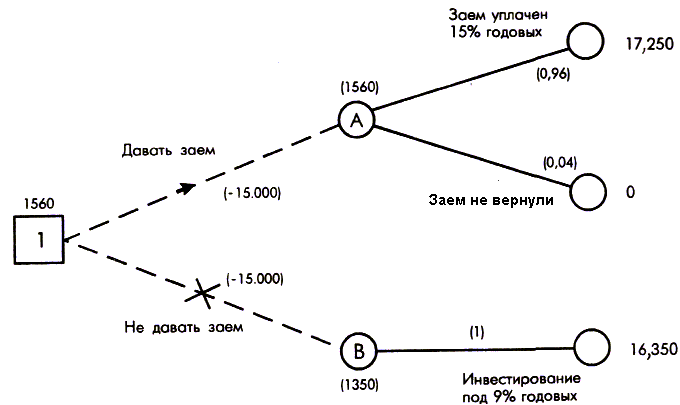
\includegraphics[height=0.4\textheight]{tree_bank.png}
		\end{center}
	  \end {itemize}
\end{frame}


\begin{frame}
\frametitle{Дополнительно}
	  \begin {itemize}
		\item Категориальные признаки можно обрабатывать, создав для каждого значения признака по потомку в дереве, а можно закодировать его средним значением целевой переменной среди элементов данного класса (Для бинарной классификации - доля обьектов). Для Джини и энтропийного критерия результат как при полном переборе. [Hastie T., Tibshirani R., Friedman J. (2009). The Elements of Statistical Learning.]
	  \end {itemize}
\end{frame}

\begin{frame}
\frametitle{Ансабли деревьев}

		Пусть есть "слабый классификатор" (угадывающий правильный ответ с вероятностью p, немного большей, чем случайный предсказатель) \\
		
		Можно ли как-то используя его, сделать "сильный классификатор"?

\end{frame}

\begin{frame}
\frametitle{Ансабли деревьев}

		Возьмём три таких классификатора, независимо угадывающих с вероятностью $p = 0.55$ и будет относить обьект к тому классу, за который проголосовало большиство. Тогда вероятность угадать класс верно равна $1 - 3 p (1 - p)^2 - p^3 = 0.57475 > p$

\end{frame}



\begin{frame}
\frametitle{Ансабли деревьев}

        Проблема в том, что деревья строятся не случайно (алгоритм, описанный выше детерменирован, что, однако, верно не для всех реализаций) и тем более не независимо. Давайте модифицируем алгоритм и сделаем случайный лес из случайных деревьев.
        
\end{frame}

\begin{frame}
\frametitle{Bootstrap}
        \begin{rudef}
            Пусть дана выборка X из n обьектов. Выберем несколько раз, например n, равновероятно случайный обьект из X (выбор с повторениями). Выборку составленную из этих обьектов назовём bootstrap-выборкой.
        \end{rudef}
        
        Например, из [1, 2] могут получиться \\ выборки [1, 1], [1, 2], [2, 1], [2, 2].
\end{frame}

\begin{frame}
\frametitle{Случайный лес}
	  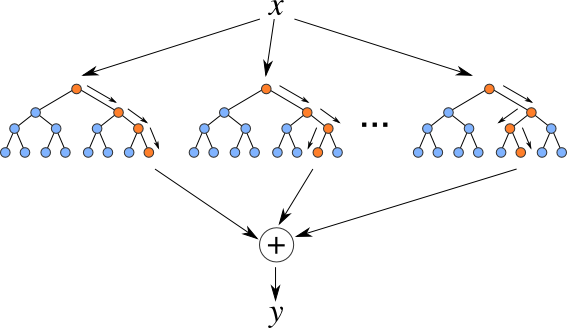
\includegraphics[width=\textwidth]{tree_rf.png}
\end{frame}

\begin{frame}
\frametitle{Случайный лес}
	  \begin {itemize}
		\item Строим случайный лес с k деревьями.
		\item Сгенерируем k bootstrap-выборок из исходной
		\item Обучим на каждой выборке своё дерево, но при построении дерева, в каждом узле дерева, будем выбирать m случайных признаков и искать оптимальное разделение только по ним (m - заранее фиксировано, например, корень от числа признаков)
		\item Ответ всего алгоритма - класс, за который проголосовало большинство или среднее для классификации и регрессии соответственно.
	  \end {itemize}
\end{frame}

\newtheorem{ruprinciple}{Принцип}

\begin{frame}
\frametitle{Bagging}
        \begin{rudef}
            В данном подходе мы агрегируем данных алгоритмов, обученных на bootstrap-выборках. В общем случае такой подход называется bagging (bootstrap aggregating).
        \end{rudef}
        
        \begin{ruprinciple}[Анны Карениной]
            Все счастливые семьи похожи друг на друга, каждая несчастливая семья несчастлива по-своему.
        \end{ruprinciple}
\end{frame}


\begin{frame}
\frametitle{Замечания}
        \begin{itemize}
            \item Предлагается строить деревья максимально грубокими, чтобы они могли выделять сложные зависимости, тогда как из-за усреднения их переобученность не будет мешать (меньше variance при усреднении, но тот же bias)
            \item На выборках, в которых пропорции классов сильно отличаются, могут возникнуть проблемы
            \item Случайный лес, не переобучается при росте числа деревьев
        \end{itemize}
\end{frame}

\begin{frame}
\frametitle{Замечания}
        \begin{itemize}
            \item При построении дерева в конкретной бутстрапной выборке не появилось около 37\% всех обьектов, поэтому для фиксированного обьекта можно оценить качество его предсказания, используя деревья, в обучении которых он не участвовал. Усредняя это качество по всем элементам исходной выборки, получим Out-Of-Bag "самооценку" качества дерева. 
            \item Также случайные леса умеют оценивать важность признаков, вычисляя feature importance.
        \end{itemize}
\end{frame}

\begin{frame}
\frametitle{Градиентный бустинг}
        \begin{rudef}
            Пусть дана функция $f(x_1...x_n)$ нескольких переменных. Её градиентом $\nabla f$ называют вектор $(\frac{\partial f(x_1...x_n)}{\partial x_1} ... \frac{\partial f(x_1...x_n)}{\partial x_n})$ её частных производных.
        \end{rudef}
        
        Градиент является направлением наискорейшего роста, тогда как противоположное направление - антиградиент - является направлением наискорейшего убывания. 
        
        
\end{frame}

\begin{frame}
\frametitle{Градиентный спуск}
        Предложим следующий алгоритм численной минимизации функции $f$:
        Выберем начальную точку $x_0$. 
        
        После этого на каждой итерации будем двигаться в направлении наискорейшего спуска:
        
        $x_{i+1} = x_{i} - \lambda_i \nabla f (x_i{})$
        
        $\lambda_i$ - шаг алгоритма, выбирается постоянным или некоторыми другими способами
\end{frame}

\begin{frame}
\frametitle{Градиентный спуск}
    \begin{center}
        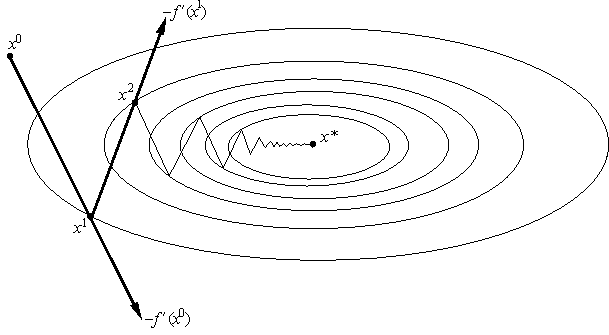
\includegraphics[width=\textheight]{tree_gradient_descent.png}
    \end{center}

\end{frame}

\begin{frame}
\frametitle{Градиентный бустинг}
    Будем строить алгоритм как $A(x) = \sum\limits_{i=0}^{n} b_i(x)$, где $b_i$ - базовые алгоритмы.
    
    Начальное приближение выбирается произвольно, например, среднее значение целевой переменной.
    $b_0(x) = \overline{y}$
    
    Пусть $L$ - функция потерь, непрерывно дифференцируемаяю

    
\end{frame}

\begin{frame}
\frametitle{Градиентный бустинг}
    Уже построили $A_{N-1}(x) = \sum\limits_{i=0}^{N - 1} b_i(x)$
    
    Задача: $\min\limits_{b_N} \sum\limits_{i=1}^{|X|} L(y_i, \sum_{i=0}^{N-1} b_i(x_i) + b_N(x_i)) $
    
    Какой сдвиг $b_N$ в пространстве алгоритмов будет давать наискорейшее убывание функции потерь?
\end{frame}


\begin{frame}
\frametitle{Градиентный бустинг}
    Ответ: такой что $b_N(x_k) = -\frac{\partial L}{\partial a}(y_1, \sum_{i=0}^{N-1} b_i(x_k))$
    
    Итого: новый алгоритм будем обучать на исходных признаках и целевых значения, указанных выше.
    Ответ обученного алгоритма на каждом шаге - сумма ответов алгоритмов, полученных на предыдущих шагах.
    
    
\end{frame}

\begin{frame}
\frametitle{Градиентный бустинг}
    Заметим, что мы осуществляем по сути градиентный спуск в пространстве алгоритмов, поэтому, как и алгоритме градиентного спуска полезно добавить множитель $\lambda$, чтобы осуществлять шаг не на всю длину градиента, а только в его направлении:
    $A_{N}(x) = \sum\limits_{i=0}^{N - 1} b_i(x) + \lambda b_N(x_i)$
    
    На практике выбор этого множителя представляет нетривиальную задачу: при большом $\lambda$ алгоритм не будет сходится, а при малом $\lambda$ алгоритм будет сходится очень медленно.

\end{frame}

\begin{frame}
\frametitle{Градиентный бустинг для MSE}
    Если $L(y, a) = (a - y) ^ 2$, то новые целевые значения, на которые обучается очередной алгоритм, вычислются очень просто: 
    $- \frac{\partial L}{\partial a} = 2 (y - a) $ 
    Так как мы ввели шаг алгоритма, то двойку можно убрать и новый алгоритм нужно обучать на вектор ошибок предыдущих алгоритмов:
    $(y_1 - A_{N-1}(x_1), ..., y_{|X|} - A_{N-1}(x_{|X|}))$ c исходными признаками. 
    
\end{frame}

\begin{frame}
\frametitle{Градиентный бустинг}
    \begin{itemize}
        \item В качестве базовых алгоритмов предлагается использовать неглубокие решающие деревья, которые можно быстро обучать.
        \item В отличие от случайного леса, алгоритм тяжело распараллеливается.
    
    \end{itemize}
    
\end{frame}

\begin{frame}
\frametitle{Градиентный бустинг}
    \begin{center}
        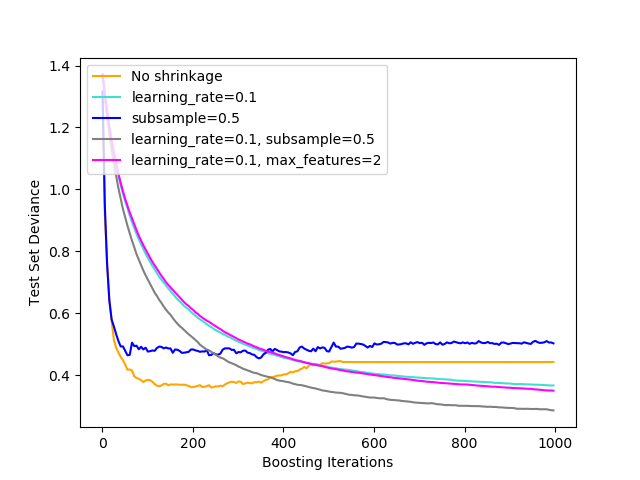
\includegraphics[width=\textheight]{tree_gb.png}
    \end{center}
\end{frame}

\begin{frame}
	\frametitle{Ссылки}
	\href{https://github.com/esokolov/ml-course-msu/blob/master/ML16/lecture-notes/Sem04_trees.pdf}{\textit{О решающих деревьях (pdf)}}\\
	\href{http://arogozhnikov.github.io/2016/06/24/gradient_boosting_explained.html}{\textit{Визуализация градиентного бустинга}}\\

\end{frame}

\end{document} 
